\section{Experiments}
\label{sec:experiments}
In the following we briefly describe the dataset we collected for the
validation of the proposed approach. Then we describe the details of
the interactive segmentation process on those data which is depicted
in Figure\ref{fig} and conclude with the actual timing of the
competing approaches.

\subsection{ALS Dataset}
\label{sec:dataset}
The data was recorded with a $3T$ scanner at Utah Brain Institute. It
consisted of $12$ ALS patients and $12$ healthy controls; $64$
gradients; $b$-value$=1000$.; anatomical scan ($1 \times 1 \times
1mm^3$).  We reconstructed the streamlines using EuDX, a deterministic
tracking algorithm ~\cite{garyfallidis2012towards} from the DiPy
library~\footnote{\url{http://www.dipy.org}}. The tractography was
then embedded in $\mathbb{R}^{p}$ using the dissimilarity
representation presented in Section~\ref{sec:dissimilarity} with
$p=40$ and the SFF prototype selection procedure as suggested
in~\cite{olivetti2012approximation}. The prototype selection and the
actual embedding of $\approx 3 \times 10^5$ streamlines required
$\approx 180$s.


\subsection{The Interactive Segmentation Process}
We describe the segmentation process following the example of the CST
segmentation in Figure~\ref{fig}. The full tractography (\ref{fig}A)
of $\approx 250000$ streamlines is initially clustered with $k=150$
and the medoids are presented to the user (1B). We observed that $150$
medoids are approximately the highest number a user can comfortably
interact with in the $3$D scene when the whole tractography is
presented. Then user selects $20$ clusters by clicking on the
corresponding medoids (\ref{fig}B, in white). These clusters
correspond to a set of $\approx 15000$ streamlines (\ref{fig}C). These
streamlines are re-clustered into $k=50$ clusters (\ref{fig}D) and the
user selects $25$ of them (\ref{fig}D, in white). We observed that
$50$ medoids are approximately the highest number a user can
comfortably interact with after the initial selection from the full
tractography. The $25$ selected clusters corresponds to $\approx 3000$
streamlines (\ref{fig}E) that are then re-clustered into $k=50$
clusters (\ref{fig}F). In two further steps the user reduces the
selected streamlines to $\approx 1500$ (\ref{fig}G) and then to
$\approx 500$ (\ref{fig}I) thus reaching the desired segmentation of
the CST. We observed that a trained neuroanatomist could segment the
CST in approximately in $5$ minutes.

The average timings of the clustering algorithms of
Section~\ref{sec:methods} are reported in Table~\ref{tab:results}. In
the first column (size) are reported the size of the subset of
streamlines that we considered of practical use. The second column
($k$) reports the number of clusters. The third ($k$-means) and the
fourth (MBKM) reports the time for clustering. The Fifth column
reports the size ($b$) of the mini-batches for the MBKM, which was
always $100$ except for the full tractography for which we observed a
significant gain in time when increasing it to $1000$. The sixth
column reports the time to compute the medoids after clustering, which
was always negligible with respect to the clustering time.

The tractography segmentation tool was implemented in Python code on
top of the DiPy, Fos~\footnote{\url{http://fos.me}} and
OpenGL~\footnote{\url{http://opengl.org}}. The free software project
of the segmentation tool, currently in alpha stage, is hosted within
the DiPy project. The code of the dissimilarity representation is
from~\cite{olivetti2012approximation}~\footnote{\url{https://github.com/emanuele/prni2012_dissimilarity}}
and that of the $k$-means, the MBKM and the $k$-means++ is from
scikit-learn~\cite{pedregosa2011scikit}~\footnote{http://scikit-learn.org}.

\begin{figure*}[t]
\centering
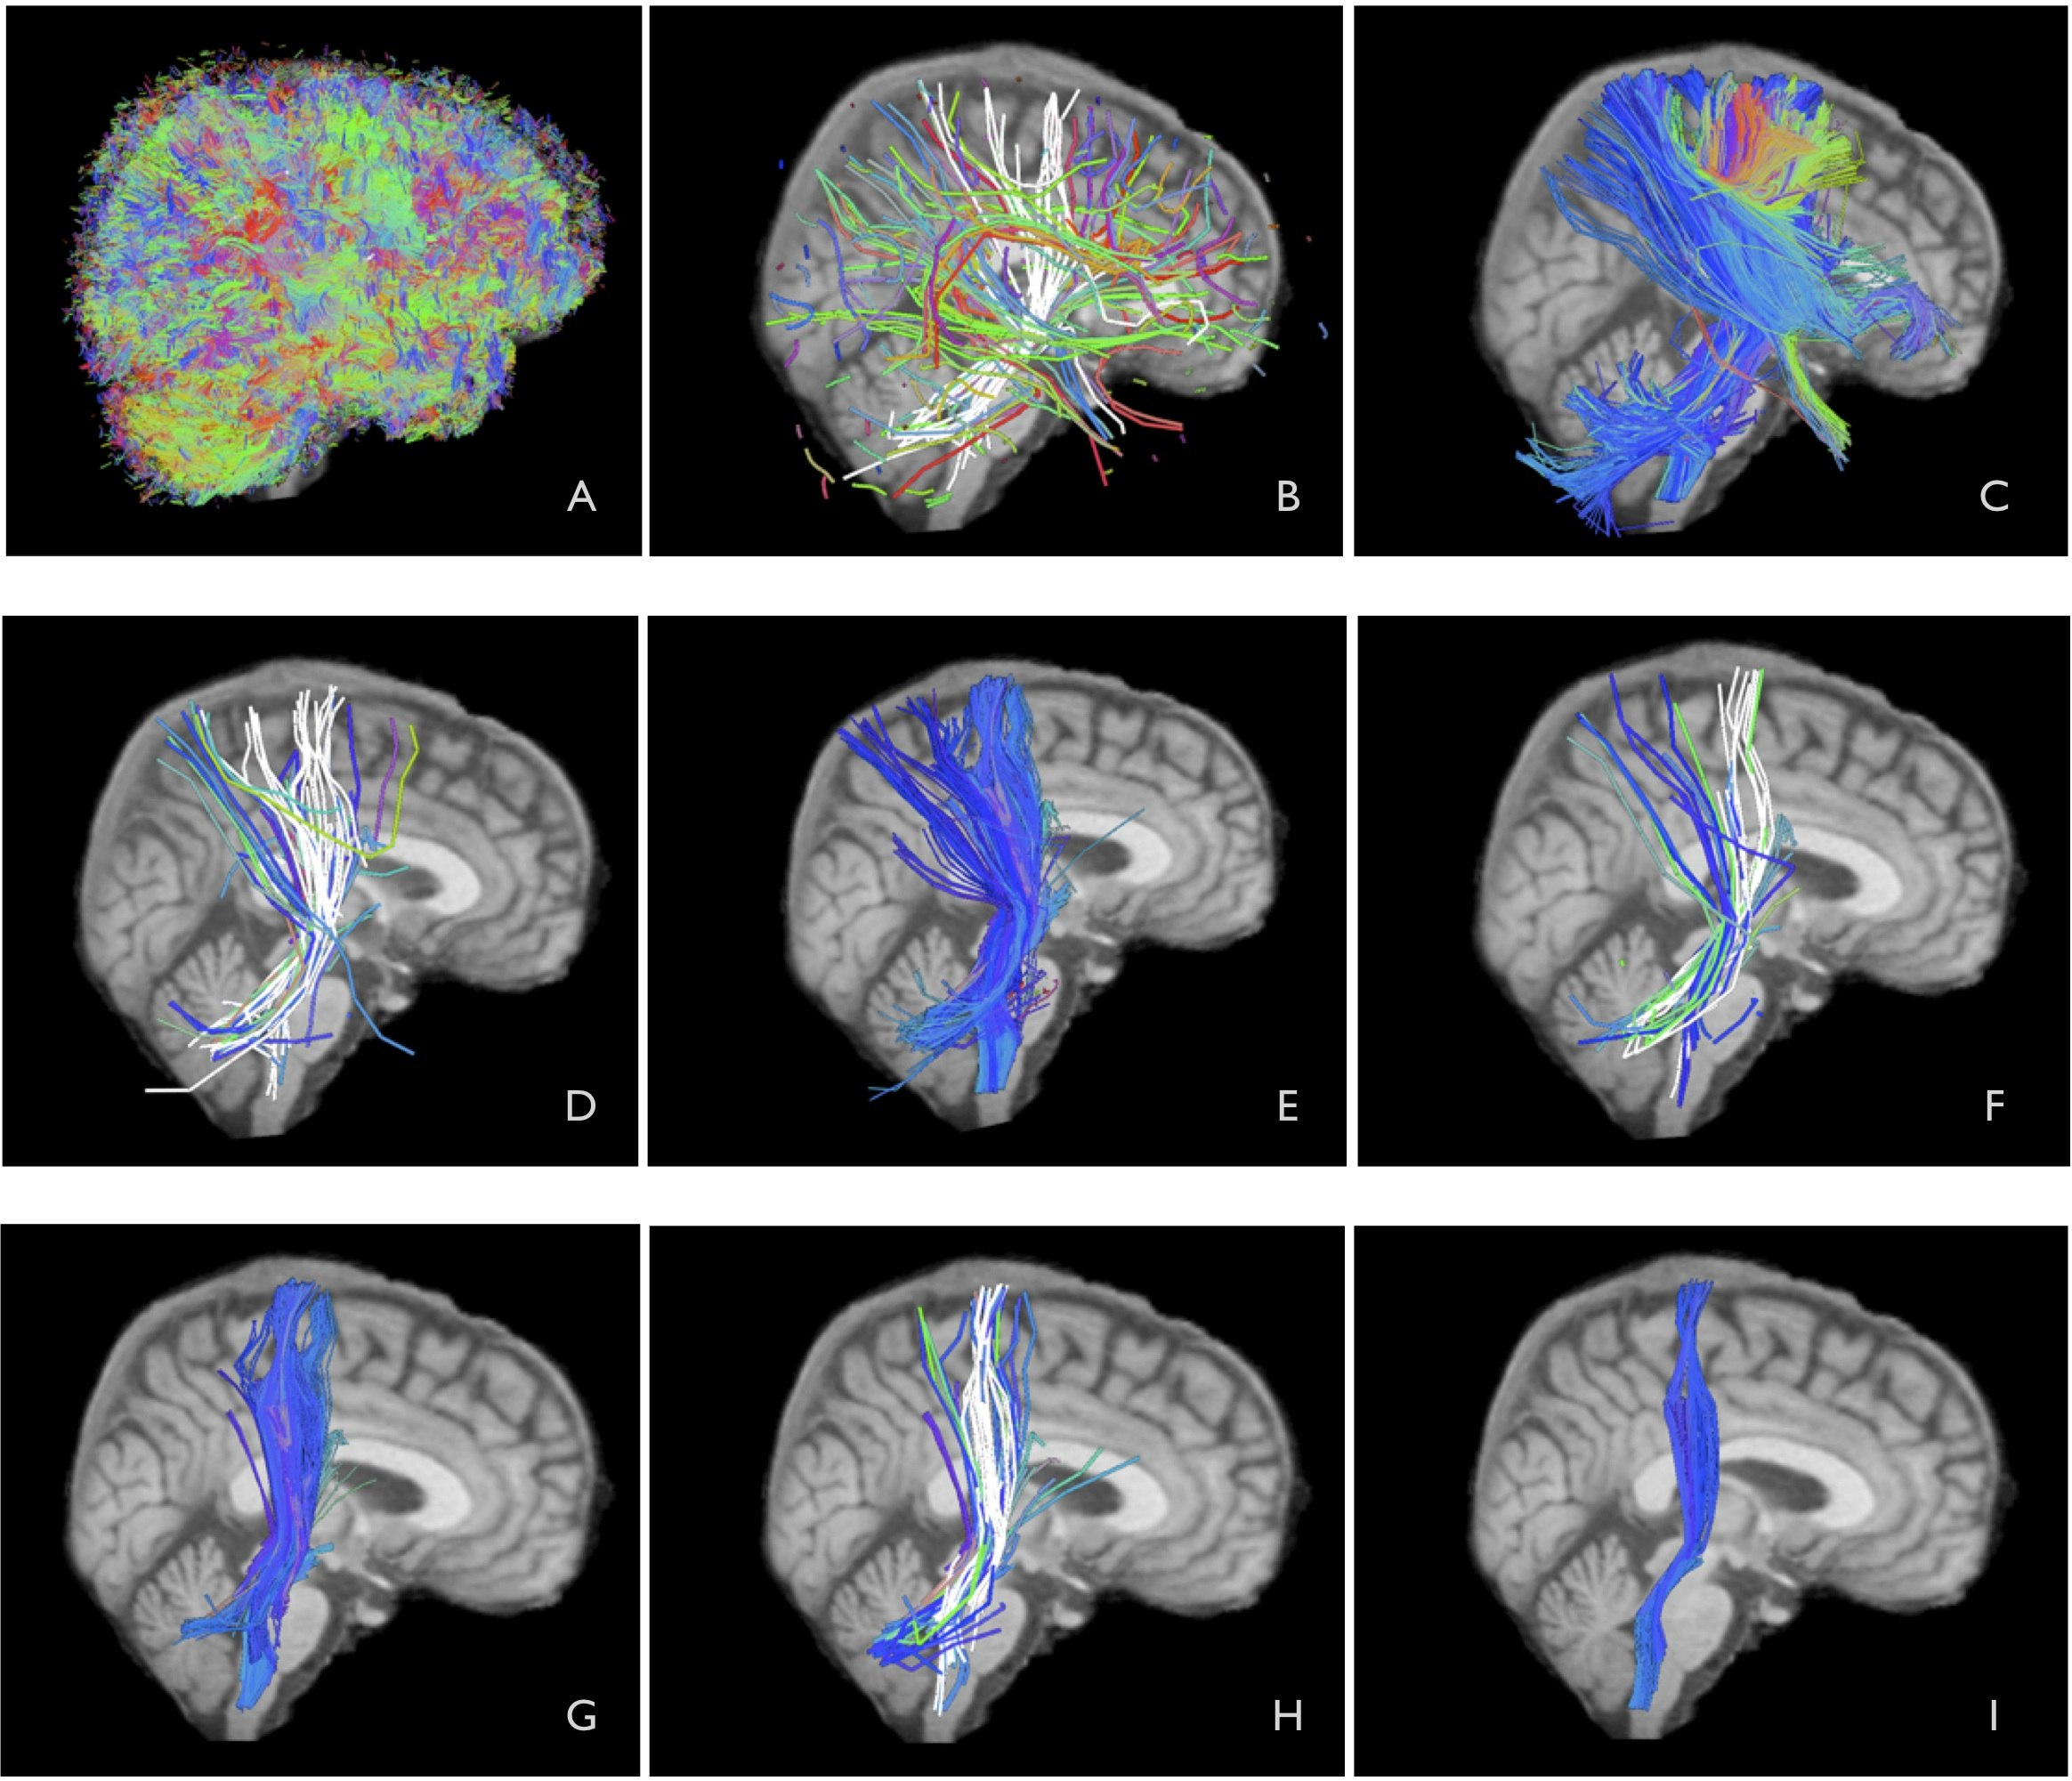
\includegraphics[width=\textwidth]{figure}
\caption{Segmentation Process. (A) Full tractography $\approx$300K
  streamlines; (B) Computation of 150 clusters and selection of $\approx$20 clusters; (C)
  $\approx$15k streamlines corresponding to selection; (D) Computation of ~50
  clusters and selection of $\approx$25
  clusters; (E) $\approx$3K streamlines corresponding to
  selection; (F) Computation of 50 clusters and selection of $\approx$15
  clusters; ( G) $\approx$1.5K streamlines corresponding to selection; (H)
  Computation of 50 clusters and selection of $\approx$25 clusters; (I) $\approx$500
  streamlines corresponding to selection and representing the
  corticospinal tract.}
\label{fig}
\end{figure*}


\begin{table}
  \centering
  \begin{tabular}{ r | r || c | c || c || c }
    size & $k$ & $k$-means & MBKM & b &  medoids \\
    \hline
    \hline
    $500$    &  $50$ &  $0.3s$ &  $\mathbf{0.2}s$ &  $100$ &  $0.003s$ \\
    \hline
    $1000$   &  $50$ &  $0.6s$ &  $\mathbf{0.2}s$ &  $100$ &  $0.004s$ \\
    \hline
    $5000$   &  $50$ &  $6.1s$ &  $\mathbf{0.4}s$ &  $100$ &  $0.007s$ \\
    \hline
    $10000$  &  $50$ & $14.4s$ &  $\mathbf{0.6}s$ & $100$ &   $0.011s$ \\
    \hline
    $15000$  &  $50$ & $29.9s$ &  $\mathbf{0.7}s$ & $100$ &  $0.016s$ \\
    \hline
    $250000$ & $150$ & $>1000s$ & $\mathbf{13.3}s$ &  $1000$  &  $0.151s$ \\
    \hline
  \end{tabular}
  \caption{Clusterning results.}
  \label{tab:results}
\end{table}

%%% Local Variables: 
%%% mode: latex
%%% TeX-master: "olivetti_boi"
%%% End: 

